%%%%%%%%%%%%%%%%%%%%%%%%%%%%%%%%%%%%%%%%%%%%%%%%%%%%%%%%%%%%%%%%%%%%%%%%%
% sample poster file 
%%%%%%%%%%%%%%%%%%%%%%%%%%%%%%%%%%%%%%%%%%%%%%%%%%%%%%%%%%%%%%%%%%%%%%%%%

%%%%%%%%%%%%%%%%%%%%%%%%%%%%%%%%%%%%%%%%%%%%%%%%%%%%%%%%%%%%%%%%%%%%%%%%%
%% IGL Template
% Last modified: Tue 19 Feb 2013 02:42:39 PM CST
%%%%%%%%%%%%%%%%%%%%%%%%%%%%%%%%%%%%%%%%%%%%%%%%%%%%%%%%%%%%%%%%%%%%%%%%%


%%%%%%%%%%%%%%%%%%%%%%%%%%%%%%%%%%%%%%%%%%%%%%%%%%%%%%%%%%%%%%%%%%%%%%%%%
% documentclass option: pick one:
% "presentation" for powerpoint-like talk,
% "handout" for  printing,
% "trans" for printing onto transparencies
%%%%%%%%%%%%%%%%%%%%%%%%%%%%%%%%%%%%%%%%%%%%%%%%%%%%%%%%%%%%%%%%%%%%%%%%%


%\documentclass[leqno,presentation]{beamer}
\documentclass[leqno, handout]{beamer}
%\documentclass[leqno,trans]{beamer}


%%%%%%%%%%%%%%%%%%%%%%%%%%%%%%%%%%%%%%%%%%%%%%%%%%%%%%%%%%%%%%%%%%%%%%%%%
% beamerposter stuff
%%%%%%%%%%%%%%%%%%%%%%%%%%%%%%%%%%%%%%%%%%%%%%%%%%%%%%%%%%%%%%%%%%%%%%%%%
\usepackage[orientation=landscape, size=a0, scale=1.3]{beamerposter}
\usepackage{pgf}
\usepackage{tikz}
% these packages may be needed 
\usepackage{calc}
\usepackage{times}
\usepackage{type1cm}
\usepackage[latin1]{inputenc}

%%%%%%%%%%%%%%%%%%%%%%%%%%%%%%%%%%%%%%%%%%%%%%%%%%%%%%%%%%%%%%%%%%%%%%%%%
% end beamerposter stuff
%%%%%%%%%%%%%%%%%%%%%%%%%%%%%%%%%%%%%%%%%%%%%%%%%%%%%%%%%%%%%%%%%%%%%%%%%


% load standard packages

\usepackage{amsmath,amssymb, latexsym}
\usepackage[english]{babel}


%\usepackage{hyperref}
%\hypersetup{pdfborderstyle={/S/U/W },pdfborder=0 0 1}

%\usepackage{graphicx}
%\DeclareGraphicsExtensions{.eps, .pdf,.jpg,.png, .tif}

%%%%%%%%%%%%%%%%%%%%%%%%%%%%%%%%%%%%%%%%%%%%%%%%%%%%%%%%%%%%%%%%%%%%%%%%%
% theme
%%%%%%%%%%%%%%%%%%%%%%%%%%%%%%%%%%%%%%%%%%%%%%%%%%%%%%%%%%%%%%%%%%%%%%%%%


%% this seems to work fine

\usetheme{Darmstadt}

%\usetheme{Singapore}


%% beamerposter example uses Berlin, but couldn't get rid of footers 

%\usetheme{Berlin}
%\usetheme{Warsaw}


%\usetheme{PaloAlto}
%\usetheme{AnnArbor}
%\usetheme{CambridgeUS}
%\usetheme{CambridgeUS}
%\usetheme{Berkeley}
%\usetheme{Madrid}


%%%%%%%%%%%%%%%%%%%%%%%%%%%%%%%%%%%%%%%%%%%%%%%%%%%%%%%%%%%%%%%%%%%%%%%%%
%%%%%%%%%%%%%%%%%%%%%%%%%%%%%%%%%%%%%%%%%%%%%%%%%%%%%%%%%%%%%%%%%%%%%%%%%
% begin macros
%%%%%%%%%%%%%%%%%%%%%%%%%%%%%%%%%%%%%%%%%%%%%%%%%%%%%%%%%%%%%%%%%%%%%%%%%
%%%%%%%%%%%%%%%%%%%%%%%%%%%%%%%%%%%%%%%%%%%%%%%%%%%%%%%%%%%%%%%%%%%%%%%%%


% theorem declarations

%\newtheorem{question1}{Question 1}
%\newtheorem{question2}{Question 2}

\theoremstyle{definition}
%\newtheorem{brokenstickproblem}{Broken Stick Problem}




%%%%%%%%%%%%%%%%%%%%%%%%%%%%%%%%%%%%%%%%%%%%%%%%%%%%%%%%%%%%%%%%%%%%%%%%%
%%%%%%%%%%%%%%%%%%%%%%%%%%%%%%%%%%%%%%%%%%%%%%%%%%%%%%%%%%%%%%%%%%%%%%%%%
% end macros
%%%%%%%%%%%%%%%%%%%%%%%%%%%%%%%%%%%%%%%%%%%%%%%%%%%%%%%%%%%%%%%%%%%%%%%%%
%%%%%%%%%%%%%%%%%%%%%%%%%%%%%%%%%%%%%%%%%%%%%%%%%%%%%%%%%%%%%%%%%%%%%%%%%

%%%%%%%%%%%%%%%%%%%%%%%%%%%%%%%%%%%%%%%%%%%%%%%%%%%%%%%%%%%%%%%%%%%%%%%%%
% title/author/date
%%%%%%%%%%%%%%%%%%%%%%%%%%%%%%%%%%%%%%%%%%%%%%%%%%%%%%%%%%%%%%%%%%%%%%%%%

%% size up title and author for poster 

\title{
\veryHuge
Mathematics of Gerrymandering}
  \author{
  \LARGE
Weifan Jiang, Namyoung Kim, Alex Robkin, Leo Segovia, Faculty Mentor: Chris Hoffman, Graduate Mentor: Tejas Devanur}
  

%% uiuc and igl logos DON'T CHANGE ANYTHING HERE
%\institute{
%\raisebox{-2ex}{\includegraphics[width=5in]{uwletterhead1.png}}
%\hspace{4em}
%\raisebox{-2ex}{\includegraphics[width=1in]{LogoPDF.pdf}}
%\hspace{1em} 
%\raisebox{-2ex}{\includegraphics[width=1in]{primesLogo100.jpg}}
%\hspace{1em} 
%{\Large\textcolor{red!50!blue}{ Washington Experimental Mathematics Lab and MIT-PRIMES}}
%}


\date{\large Winter 2018}



%% logo, shows up  in top left corner of each frame
%\logo{%
%\includegraphics[width=0.4in]{igl-logo-small.png}
%}


%%%%%%%%%%%%%%%%%%%%%%%%%%%%%%%%%%%%%%%%%%%%%%%%%%%%%%%%%%%%%%%%%%%%%%%%%


\begin{document}
\begin{frame}

%%%%%%%%%%%%%%%%%%%%%%%%%%%%%%%%%%%%%%%%%%%%%%%%%%%%%%%%%%%%%%%%%%%%%%%%%
% title frame 
%%%%%%%%%%%%%%%%%%%%%%%%%%%%%%%%%%%%%%%%%%%%%%%%%%%%%%%%%%%%%%%%%%%%%%%%%

\begin{block}{}
\titlepage
\end{block}

%%%%%%%%%%%%%%%%%%%%%%%%%%%%%%%%%%%%%%%%%%%%%%%%%%%%%%%%%%%%%%%%%%%%%%%%%
% body of poster
%%%%%%%%%%%%%%%%%%%%%%%%%%%%%%%%%%%%%%%%%%%%%%%%%%%%%%%%%%%%%%%%%%%%%%%%%

\begin{columns}[t]

%%%%%%%%%%%%%%%%%%%%%%%%%%%%%%%%%%%%%%%%%%%%%%%%%%%%%%%%%%%%%%%%%%%%%%%%%
% left column
%%%%%%%%%%%%%%%%%%%%%%%%%%%%%%%%%%%%%%%%%%%%%%%%%%%%%%%%%%%%%%%%%%%%%%%%%

\begin{column}[t]{.25\linewidth}

%%%%%%%%%%%%%%%%%%%%%%%%%%%%%%%%%%%%%%
% left block 1
%%%%%%%%%%%%%%%%%%%%%%%%%%%%%%%%%%%%%%
\begin{block}{Motivation}
This research focuses on the mathematics of gerrymandering.
Gerrymandering refers to how political parties draw district
boundaries to give them better odds at receiving a majority during
congressional elections. Every 10 years, local district boundaries in the
United States are redrawn for congressional elections by the current
majority party for each state. With such change in political cartography, redrawing district boundaries not only affects who wins but also the people who live within them. With such loosely defined criteria for
redistricting, we seek to quantify the process of redrawing district
lines to determine when this partisan process becomes an act of
manipulation and exclusion.    
% \begin{itemize}
%  \item Apollonius (2nd century BCE)---discovered that given three mutually tangent circles, exactly two circles are tangent to all three
%  \item Rene Descartes (17th century CE)---related the radii of three mutually tangent circles and a fourth that is outside and tangent to the original three
%  \item Frederick Soddy (1937)---rediscovered Descartes' formula and extended to three-dimensions
% \end{itemize}

\end{block}
%%%%%%%%%%%%%%%%%%%%%%%%%%%%%%%%%%%%%%
% end left block 1
%%%%%%%%%%%%%%%%%%%%%%%%%%%%%%%%%%%%%%

%%%%%%%%%%%%%%%%%%%%%%%%%%%%%%%%%%%%%%
% left block 2
%%%%%%%%%%%%%%%%%%%%%%%%%%%%%%%%%%%%%%
\begin{block}{The Metropolis-Hastings Algorithm}
We will be using the The Metropolis Hastings (M.H.) algorithm to produce a random walk that has as its unique stationary distribution the ideal probability distribution, $p$, of all possible districting plans for a given U.S state.
We begin with an arbitrary sample in our distribution, $x_0$. We then choose at random a different sample that is maximally similar to $x_0$, $x^*$. We then choose $x_1=x^*$ with probability min$(1, \frac{p(x^*)}{p(x_0)})$ and otherwise choose $x_1=x_0$. We repeat this process for several iterations.     
% \ 

% Last semester, we considered properties of this packing. We made pictures to help visualize the following problems: if we take another horizontal line at height $h$, what proportion of the line that is contained in the circles of the Farey-Ford packing?  What is the limit of this proportion as the horizontal line approaches the $x$-axis?
\end{block}
%%%%%%%%%%%%%%%%%%%%%%%%%%%%%%%%%%%%%%
% end left block 2
%%%%%%%%%%%%%%%%%%%%%%%%%%%%%%%%%%%%%%

%%%%%%%%%%%%%%%%%%%%%%%%%%%%%%%%%%%%%%
% left block 3
%%%%%%%%%%%%%%%%%%%%%%%%%%%%%%%%%%%%%%
\begin{block}{Iowa}
By collecting congressional maps and election results, we
implemented the M.H. algorithm in python to produce a sample space for Iowa. The random walk model considers local
and federal redistricting requirements using self-defined parameters which measure: compactness of districts and population division. 

% \ 

% This semester, we looked at the analog of the problem we considered last semester. We considered what proportion of the plane $z=h$ intersects with the spheres tangent to the plane $z=0$ and the limit of this proportion as $h$ approaches $0$.
\end{block}
%%%%%%%%%%%%%%%%%%%%%%%%%%%%%%%%%%%%%%
% end left block 3
%%%%%%%%%%%%%%%%%%%%%%%%%%%%%%%%%%%%%%


\end{column}

%%%%%%%%%%%%%%%%%%%%%%%%%%%%%%%%%%%%%%%%%%%%%%%%%%%%%%%%%%%%%%%%%%%%%%%%%
% end left column
%%%%%%%%%%%%%%%%%%%%%%%%%%%%%%%%%%%%%%%%%%%%%%%%%%%%%%%%%%%%%%%%%%%%%%%%%


%%%%%%%%%%%%%%%%%%%%%%%%%%%%%%%%%%%%%%%%%%%%%%%%%%%%%%%%%%%%%%%%%%%%%%%%%
% middle column, wide
%%%%%%%%%%%%%%%%%%%%%%%%%%%%%%%%%%%%%%%%%%%%%%%%%%%%%%%%%%%%%%%%%%%%%%%%%

\begin{column}{.45\linewidth}

%%%%%%%%%%%%%%%%%%%%%%%%%%%%%%%%%%%%%%
% center block 1
%%%%%%%%%%%%%%%%%%%%%%%%%%%%%%%%%%%%%%
%\begin{block}
%\end{block}
\begin{columns}[t]
\begin{column}{.48\linewidth}
\begin{block}{District Maps}
\vspace{1ex}
\begin{figure}
		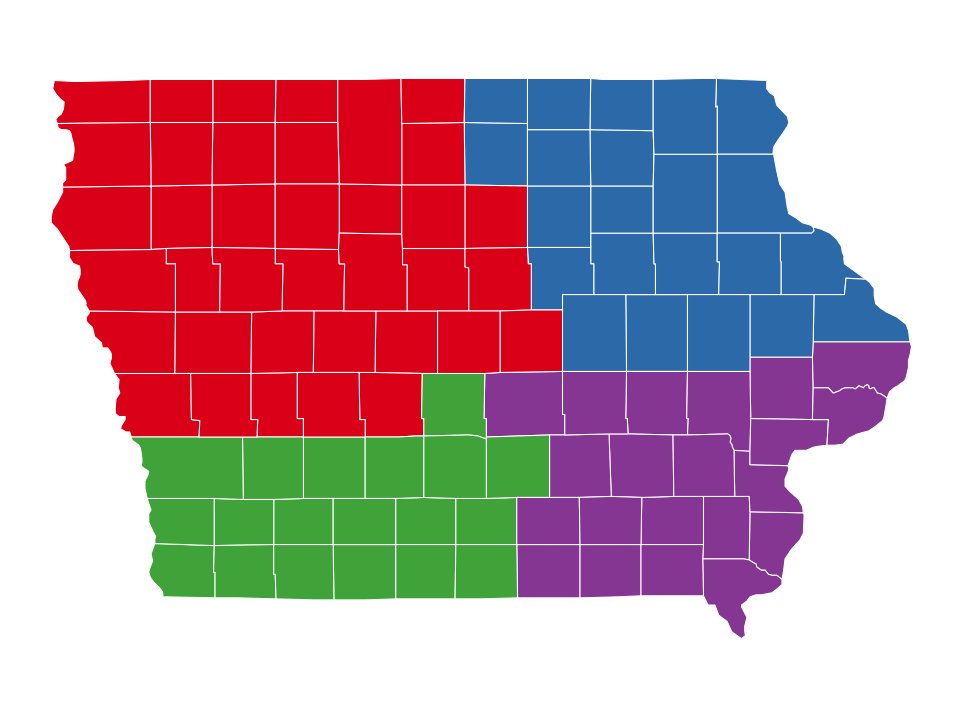
\includegraphics[width=25cm]{redistricting7.png}\\
		\caption{Above is a sample redistricting plan generated by our algorithm.}
		\end{figure}

\begin{figure}
		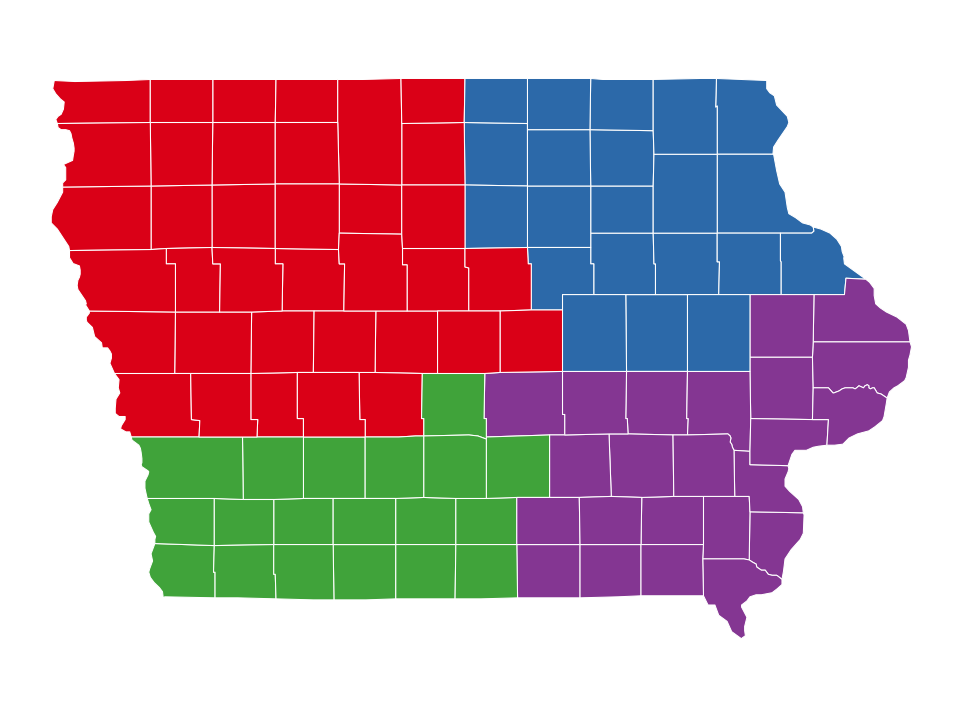
\includegraphics[width=25cm]{redistricting9.png}\\
		\caption{Above is a sample redistricting plan generated by our algorithm.}
		\end{figure}

%\begin{figure}
%		\includegraphics[width=25cm]{hhh.jpg}\\
		%\caption{}
		%\end{figure}


\end{block}
\end{column}


\begin{column}[t]{.48\linewidth}
\begin{block}{Election Simulations}
\begin{figure}
		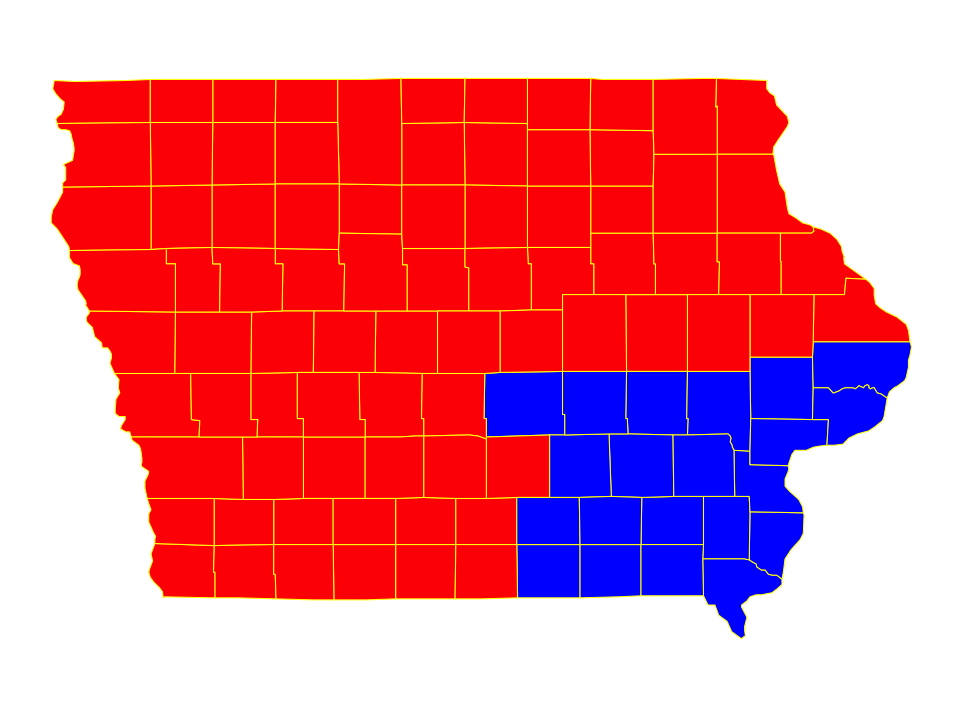
\includegraphics[width=25cm]{simulation7.png}\\
		\caption{Above is a result of election simulation corresponding to the left redistricting plan by using 2016 presidential election data. Republicans won in the three red districts and Democratics only won in the one blue district. }
		\end{figure}

\begin{figure}
		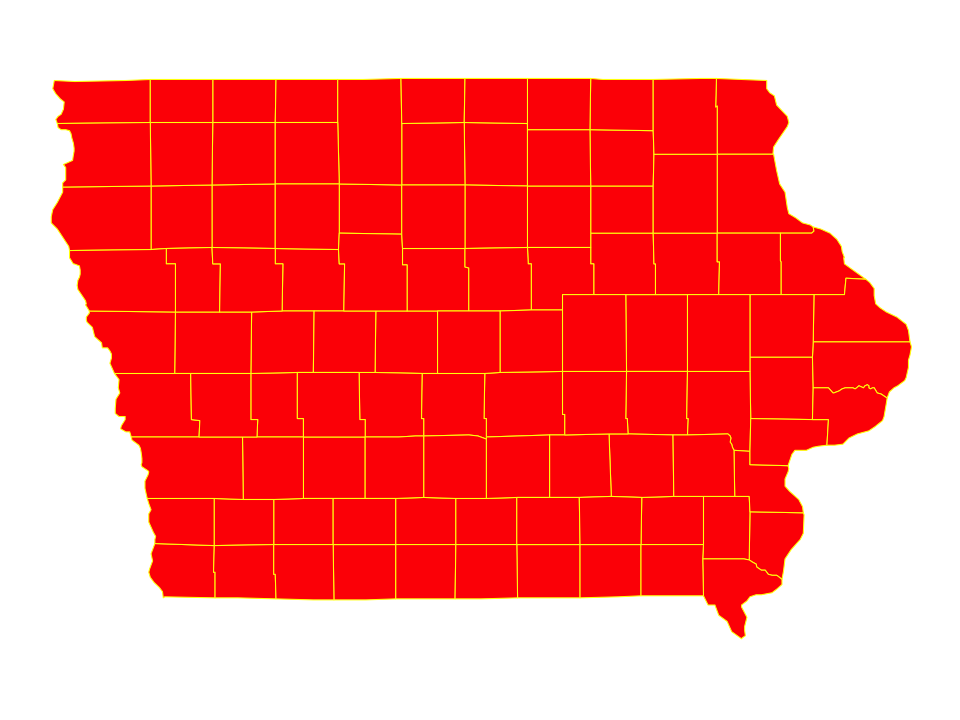
\includegraphics[width=25cm]{simulation9.png}\\
		\caption{Above is a result of election simulation corresponding to the left redistricting plan by using 2016 presidential election data. Republicans won in every district. }
		\end{figure}


\end{block}
\end{column}
\end{columns}
%\end{block}
%%%%%%%%%%%%%%%%%%%%%%%%%%%%%%%%%%%%%%
% end center block 1
%%%%%%%%%%%%%%%%%%%%%%%%%%%%%%%%%%%%%%


\end{column}

%%%%%%%%%%%%%%%%%%%%%%%%%%%%%%%%%%%%%%%%%%%%%%%%%%%%%%%%%%%%%%%%%%%%%%%%%
% end middle column, wide
%%%%%%%%%%%%%%%%%%%%%%%%%%%%%%%%%%%%%%%%%%%%%%%%%%%%%%%%%%%%%%%%%%%%%%%%%


%%%%%%%%%%%%%%%%%%%%%%%%%%%%%%%%%%%%%%%%%%%%%%%%%%%%%%%%%%%%%%%%%%%%%%%%%
% right column, narrow 
%%%%%%%%%%%%%%%%%%%%%%%%%%%%%%%%%%%%%%%%%%%%%%%%%%%%%%%%%%%%%%%%%%%%%%%%%

\begin{column}{.25\linewidth}

%%%%%%%%%%%%%%%%%%%%%%%%%%%%%%%%%%%%%%
% right block 1
%%%%%%%%%%%%%%%%%%%%%%%%%%%%%%%%%%%%%%
\begin{block}{Energies for Iowa}
Population energy:
\[\sum_{Districts}\left(\text{District Pop.}- \frac{\text{State pop.}}{\text{Number of districts}}\right)^2\]
Compactness energy:
\[\sum_{Districts}\frac{\text{(District perimeter)}^2}{\text{District area}}\]
Accept candidate with probability:
\[\text{min}\left(1,\frac{\textnormal{exp(weighted sum of current energies})}{\textnormal{exp(weighted sum of candidate energies})}\right)\]

% From the plot in the bottom-left, it appears that the proportion of the line $y=h$ that intersects the Farey-Ford packing approaches $\frac{3}{\pi}$ as $h$ drops to zero. When we plot the error of our approximation (calculated proportion minus expected value), the proportion of the line that is red very quickly approaches what we know is the true value. 

% \ 

% If we were to further plot the logarithm of this error at height $h$ divided by the logarithm of $h$, the resulting plot appears to be bounded by the constant $\frac{3}{2}$. If we could show that the plot truly is bounded by $\frac{3}{2}$, it would prove the Riemann Hypothesis. 

% \ 

% In the three-dimensional analog, we can again calculate the proportion of a plane (by use of a triangular section) that is included in the sphere packing. The bottom-right picture shows our data.  As the height of the plane approaches 0, our value seems to approach a specific limit, whose value we estimate at $0.852$. At $h=.01$, the ratio is $\approx 0.853324$.
\end{block}
%%%%%%%%%%%%%%%%%%%%%%%%%%%%%%%%%%%%%%
% end right block 1
%%%%%%%%%%%%%%%%%%%%%%%%%%%%%%%%%%%%%%

%%%%%%%%%%%%%%%%%%%%%%%%%%%%%%%%%%%%%%
% right block 2
%%%%%%%%%%%%%%%%%%%%%%%%%%%%%%%%%%%%%%
\begin{block}{Future Work}
We will define majority-minority energy equation in a way that ensures minorities have an equal opportunity to elect representatives of their choice. We will also define the counties-split energy equation where division of boundaries of cities and counties should be minimized. 

Ultimately, our goal is to simulate election results with respect to our sample districts
and compare the simulated outcomes with actual district maps and their
election results.

This study will help to determine if the current redrawn maps legitimately reflect the people they purport to represent. The next state we will be applying our model to will be the state of Washington.
\end{block}
%%%%%%%%%%%%%%%%%%%%%%%%%%%%%%%%%%%%%%
% end right block 2
%%%%%%%%%%%%%%%%%%%%%%%%%%%%%%%%%%%%%%

%%%%%%%%%%%%%%%%%%%%%%%%%%%%%%%%%%%%%%
% right block 3
%%%%%%%%%%%%%%%%%%%%%%%%%%%%%%%%%%%%%%
\begin{block}{References}
Bangia, S., Dou, B., Guo, S., Mattingly, J., \& Vaughn, C. (n.d.). Quantifying Gerrymandering.
% \begin{itemize}
% \item Athreya, J., Boca, F., and Zaharescu, A. ``Radial density in Apollonian circle packings.'' In preparation.

% \item Kontorovich, A. ``The Local-Global Principle for Integral Soddy Sphere Packings.'' arXiv:1208.5441.

% \item Marden, A. \emph{Outer circles: an introduction to hyperbolic 3-manifolds.} Cambridge: Cambridge University Press, 2007.
% \end{itemize}
\end{block}
%%%%%%%%%%%%%%%%%%%%%%%%%%%%%%%%%%%%%%
% end right block 3
%%%%%%%%%%%%%%%%%%%%%%%%%%%%%%%%%%%%%%

\end{column}
%%%%%%%%%%%%%%%%%%%%%%%%%%%%%%%%%%%%%%%%%%%%%%%%%%%%%%%%%%%%%%%%%%%%%%%%%
% end right column
%%%%%%%%%%%%%%%%%%%%%%%%%%%%%%%%%%%%%%%%%%%%%%%%%%%%%%%%%%%%%%%%%%%%%%%%%

\end{columns}
%%%%%%%%%%%%%%%
%Funding Acknowledgements: Make sure you get this right before sending to printers
%%%%%%%%%%%%%%%

\vfill

  \begin{block}{}
   \begin{center}
%    This poster is made with support from the Department of Mathematics and the Public Engagement Office at the University of Illinois at Urbana-Champaign.
  \end{center}
  \end{block}



\end{frame}
\end{document}

